%!TEX root = project.tex

\chapter{Methodology}

For the project we used the waterfall methodology. We started by mapping out the requirements for the project. Then we designed how the UI would be implemented, how the user should be able to add an account on the system.  We used GitHub for source control of the program, we also used overleaf for collaboration with the dissertation. 

\newpage
\section{Requirements}

We mapped out the requirements of our project:
\begin{itemize}
\item We would need a server or some form of central point that connects the users to any back-end that we \item would require too run the game.
\item We decided the system required a login system that would allow a user to create an account or login to an existing one.
\item We then would need a system that allowed players to connect to other users.
\item We would need a lobby systems where players can wait for a game to start or wait for other players to join the game.
\item Once the game has ended we would need a system that could keep track of the players games and achievements such as a scoreboard system.
\end{itemize}


The game Itself:
\begin{itemize}
\item Must have a procedural track to allow for non repetitive play.
\item Different versions of the game should connect to any instance and should not need to specify whether they can play with desktop or virtual reality headset users.
\end{itemize}

\newpage
\section{Design Stage}

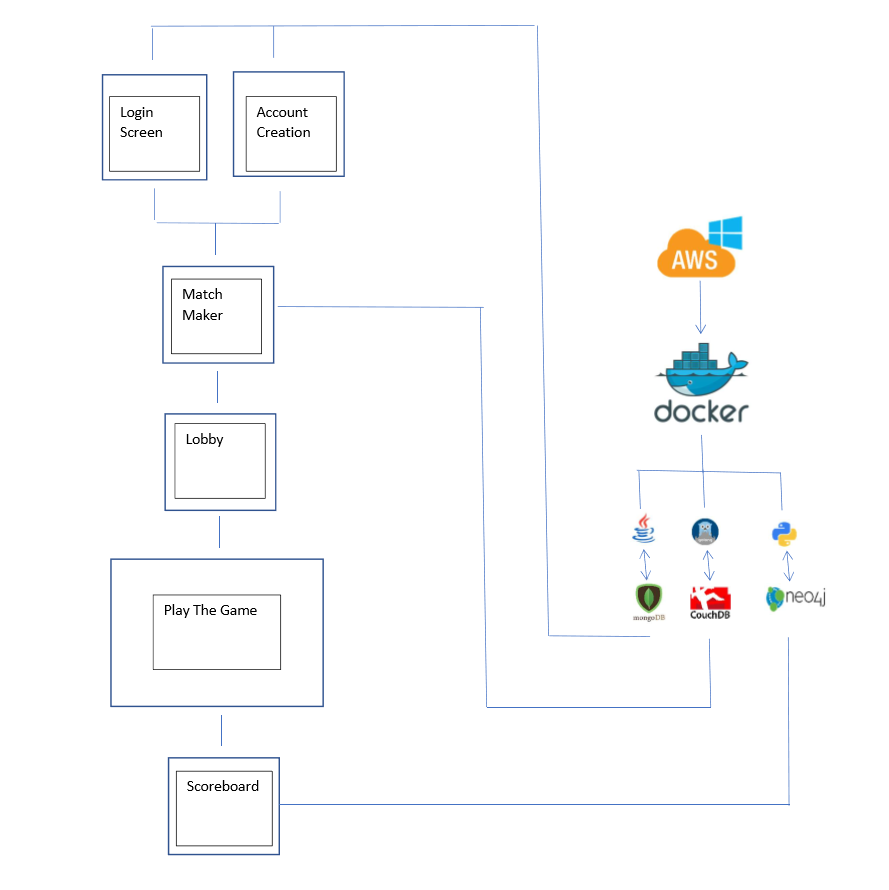
\includegraphics[width=1\columnwidth]{img/Overview.PNG}

Our login system

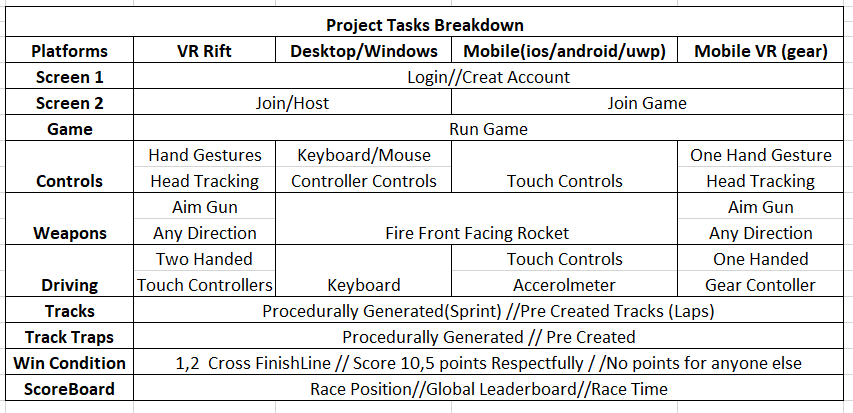
\includegraphics[width=1\columnwidth]{img/breakdown.PNG}

Our match making system

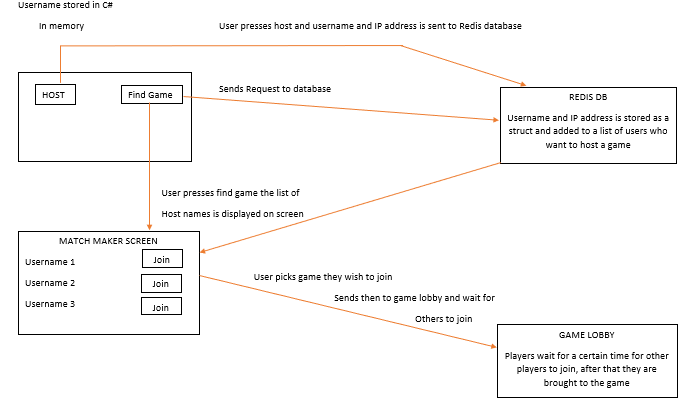
\includegraphics[width=1\columnwidth]{img/redisMatch.PNG}

An overview of the game

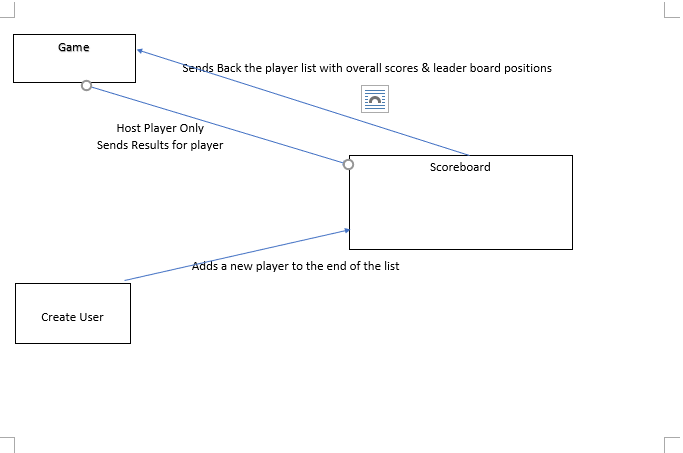
\includegraphics[width=1\columnwidth]{img/MariaDBPic.PNG}

An overview of our scoreboard system

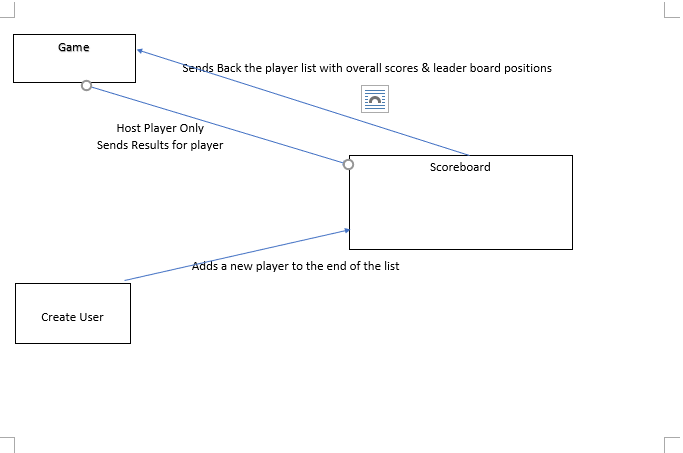
\includegraphics[width=1\columnwidth]{img/MariaDBPic.PNG}

\newpage
\section{Implementation}

\newpage
\section{Integration and System Testing}